\chapter{Introduction}\label{chapter:intro}

  \section{Membranes for Aqueous Separations}
  
  %BJC: limiting to pressure driven aqueous membrane separations (so I don't have to get into electrodialysis, gas separations, dialysis etc.)
  Pressure driven membrane processes have become an increasingly useful tool for
  performing aqueous separations. Untreated water can be a very complex solution
  with particles ranging in size from microns down to nanometers.~\cite{goosen_fouling_2005}
  Sediment, bacteria, algae, proteins, small organic molecules, and ions
  are all common components of aqueous streams.~\cite{werber_materials_2016}
  The diversity in size and chemical topology of contaminants makes the design of
  membrane processes meant to separate these components complex. To deal with 
  complex aqueous streams, and to prevent excessive membrane fouling, multiple 
  types of membranes are often used in series, removing larger particles 
  first.~\cite{suk_membranebased_2006}

  Modern membrane design is completely dependent on the target particle 
  separation. Separation membranes are most broadly classified based on the size of 
  the particle they reject. Microfiltration (MF) membranes contain pores with 
  diameters ranging from 100-10000 nm. They can separate large particles like 
  bacteria and protozoa.~\cite{ma_functionalized_2014} Ultrafiltration (UF) 
  membranes have pore diameters of about 5-500 nm and are useful for the separation
  of sugars, proteins, viruses and colloidal materials.~\cite{yanful_ultrafiltration_2009}
  Nanofiltration (NF) membranes have pores on the order of 1 nm in diameter and can 
  be used for the separation of small organic molecules and charged species.~\cite{van_der_bruggen_review_2003}
  Reverse osmosis (RO) membranes are dense amorphous polymers with tortuous 
  pathways formed by collapsed polymer networks. Their dense polymer architecture 
  rejects all solutes to a high degree except for water making them useful for 
  separating hydrated ions from water.~\cite{warsinger_review_2018} We have 
  summarized the uses of the different classes of membrane technologies in 
  Figure~\ref{fig:size_regimes}.
  
  \begin{figure}
  \centering
  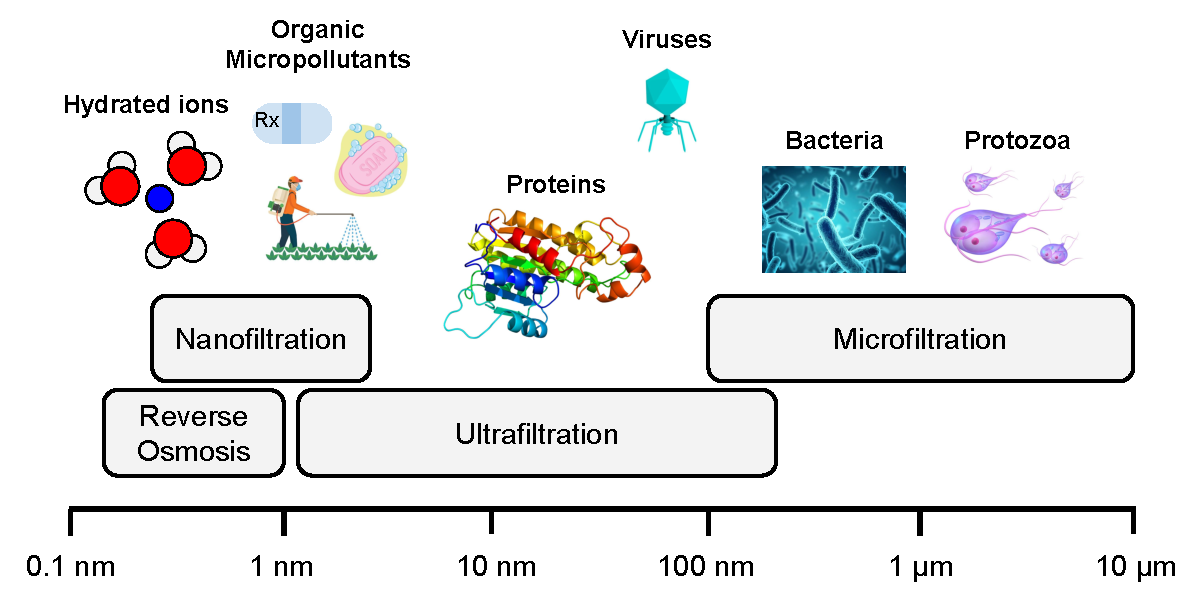
\includegraphics[width=\textwidth]{figs/membrane_separation_size_regimes.pdf}
  \caption{Choosing a membrane separation technology is entirely dependent on the
  size of the particle to be removed. The diagram provides examples of the types 
  of particles that each class of membranes is able to remove. Microfiltration (MF) 
  membranes contain pores with diameters ranging from 100-10000 nm and can separate
  large particles like bacteria and protozoa.~\cite{ma_functionalized_2014}
  Ultrafiltration (UF) membranes have pore diameters of about 5-500 nm and are 
  useful for the separation of sugars, proteins, viruses and colloidal 
  materials.~\cite{yanful_ultrafiltration_2009} Nanofiltration (NF) membranes have
  pores on the order of 1 nm in diameter and can be used for the separation of 
  small organic molecules and charged species.~\cite{van_der_bruggen_review_2003}
  Reverse osmosis (RO) membranes are dense amorphous polymers with tortuous 
  pathways formed by collapsed polymer networks. Their dense polymer architecture 
  rejects all solutes to a high degree except for water making them useful for 
  separating hydrated ions from water.~\cite{warsinger_review_2018}
  }\label{fig:size_regimes}
  \end{figure}
  
  Membranes are generally designed to optimize two key performance metrics: 
  permeability and selectivity.~\cite{geise_water_2011} Permeability is used to
  quantify the rate at which solvent and solutes pass through the membrane.
  Selectivity quantifies the relative rates of passage of two substances.
  A related quantity to selectivity, rejection, quantifies the fraction
  of undesired solute that does not pass through the membrane.
   
  Although there has been considerable focus on creating membranes with high
  permeabilities, there is a case to be made that shifting the focus to membrane
  selectivity may offer a more effective route towards lowering the cost of 
  membrane separations.~\cite{werber_materials_2016} Increasing permeabilities
  beyond those already achieved may have only a small effect on energy 
  requirements and capital costs. Cohen-Tanugi \textit{et al.} calculated that 
  a theoretical tripling of membrane permeability would only reduce energy 
  consumption by up to 15\% in a seawater RO plant.~\cite{cohen-tanugi_quantifying_2014}
  Perhaps the most aggravating influence on energy consumption is the practical
  need for multiple membrane passes in order to achieve a desired purity.~\cite{singh_production_2009}
  Additionally, many membranes are not suited for high purity separations
  of small neutral species which necessitates chemical and capital costs for
  post-treatment.~\cite{shannon_science_2009,fritzmann_state---art_2007}
  Addressing these problems with highly selective separations may lead to 
  more signficant advances.~\cite{deshmukh_desalination_2015}
  
  \subsection{Applications of Selective Membranes}
  
  Selective separations are useful in a wide range of applications. They can be used
  to separate components in both gaseous and aqueous phases.~\cite{baker_gas_2014}. We 
  will focus this section on aqueous separations since they are the target process
  for the studies that follow.
  
  \textit{Desalination}: Creating potable water from seawater or brackish water is of 
  paramount importance in water-scarce areas. It is estimated that by 2025, 1.8 
  billion people may live in water-stressed regions.~\cite{navarro-ortega_managing_2015} %There's a water stress index in fritzmann_2007
  Membrane deslination via RO and thermal muli-stage flash distillation are 
  both widely used processes for creating potable water in these regions.~\cite{fritzmann_state---art_2007}
  Compared with thermal distillation techniques, RO has been shown to 
  be more environmentally friendly and economical due to its lower energy
  requirements.\cite{morton_environmental_1997} However, thermal techniques are still
  preferred where excess waste heat or cheap thermal energy is available, such as
  cogeneration plants.\cite{bhojwani_technology_2019}

  \textit{Organic Micropollutants}: Municipal and industrial wastewaters are contaminated
  by harmful micropollutants, which can have adverse effects on human health even at low 
  concentrations.\cite{schwarzenbach_challenge_2006} Micropollutants include pharmaceuticals,
  personal care products, hormones, pesticides and industrial chemicals which find their way
  into our drinking water supply.~\cite{barbosa_occurrence_2016} Sources of micropollutants
  incude industrial wastewater, agricultural runoff, landfill leachates and domestic 
  effluents.~\cite{mompelat_occurrence_2009} Unfortunately, most waste water treatment 
  plants are not designed for complete removal of these contaminants.~\cite{tijani_review_2013}
  There is a need for a new generation of membranes that can better target specific molecules.
  
  \textit{Recovery of Valuable Dissolved Species}: In addition to removing contaminants 
  to clean waste water, we can also use highly selective membranes in order to recover
  potentially valuable dissolved species from complex municipal and industrial waste
  streams.~\cite{guest_new_2009,daigger_evolving_2009}
  
  Municipal waste-waters are rich in carbon, nitrogen and phosphorus-containing 
  compounds.~\cite{romero_raw_2013} The recovery of such products, which can be 
  achieved using selective membranes, has numerous potential uses.\cite{sales_resource_2015}
  For example, nitrogen and phosphorus recovery can help sustain fertilizer 
  production which will help meet global food demand as population continues
  to increase.\cite{xie_membrane-based_2016}

  Industrial waste-waters are often quite complex with up to six times more 
  total dissolved solids than seawater.\cite{werber_materials_2016} For example,
  flowback water, produced during hydraulic fracturing of shale formations consists
  of relatively high concentrations of salts, metals, and soluble organic 
  compounds.~\cite{orem_organic_2014} The majority of this water is disposed 
  through deep well injection, however there is a growing public concern about
  its management which has prompted the use of separation technologies such as 
  RO and NF in order to reduce the volume of contaminated water.~\cite{gregory_water_2011}
  Some of the dissolved organic compounds in flowback water, such as acetate, 
  are potentially valuable and can be recovered with highly selective membranes
  \cite{dischinger_application_2017}.

  \section{Historical Development of Membrane Technology}
  
  Membranes for separations are a relatively young technology that has expanded
  rapidly. Over the past 60 years, the field has grown into a commercially viable
  technology and the focus has shifted primarily towards incremental improvements
  in performance and most importantly, targeted separations. This section will 
  briefly cover a subset of the most relevant membrane technologies which have 
  ultimately inspired this thesis.
  
  \subsection{Reverse Osmosis Membranes}
  
  The first aqueous separations membranes were developed for RO applications 
  in the 1960s and were made of the amorphous polymer cellulose acetate (CA).~\cite{kesting_semipermeable_1965}
  Reid and Spencer were among the first to show the ability of these membranes
  to reject NaCl to high degrees ($\sim$ 99 \%) while subject to high applied 
  pressures (270 atm).~\cite{reid_ultrafiltration_1960} The most limiting 
  drawback to CA membranes is their chemical instability, undergoing severe 
  hydrolysis at pH values outside the range 4--6.~\cite{vos_kinetic_1966}
  
  Amorphous thin film composite (TFC) polyamide membranes are the current industry 
  standard for high purity RO separations.~\cite{baker_membrane_2012} Developed 
  in the 1980s, polyamide membranes are capable of rejecting salt to a higher 
  degree and can operate at wider pH ranges and higher feed pressures than 
  CA membranes.~\cite{cadotte_interfacial_1981} TFC polyamide membranes are 
  typically formed by the interfacial polymerization of a polyamide selective 
  layer on the surface of a microporous polysulfone support layer. The support
  layer gives the membrane mechanical strength without hindering the flow of 
  water thereby permitting a very thin selective layer where molecular 
  separations occur.~\cite{kucera_biofouling_2019}
  
  The dense polyamide selective layers of TFC membranes require high feed pressures,
  in the range of 5 -- 120 bar, in order to achieve a useful permeate flux.~\cite{van_der_bruggen_review_2003}
  While the energy requirements to attain these pressures are still less than 
  the energy requirements of thermal distillation\cite{morton_environmental_1997}, it 
  is often desirable to create membranes that can operate at lower feed pressures.
    %BJC2: probably could use some citations here
  It is not always necessary to achieve the high purity permeate streams
  resulting from RO. It is also possible that a target separation may be possible with 
  membranes containing larger pores. This has driven research into nanofiltration.
  
  \subsection{Nanofiltration Membranes}

  Since their introduction in the late 1980s, NF membranes have been applied towards
  an increasing number of separations since they bridge the gap in capabilities
  between reverse osmosis and ultrafiltration.~\cite{eriksson_nanofiltration_1988}
  Nanofiltration membranes have pores on the order of 1 nm in size. Larger pore sizes
  allow lower operating pressures (3 -- 20 bar) which lowers energy consumption.~\cite{van_der_bruggen_review_2003}
  An ideal NF membrane should have densely packed, uniform-sized and non-tortuous 
  pores.~\cite{jackson_nanoporous_2010} This combination has been practically difficult to realize.
  
  The most widely used methods of NF membrane fabrication are interfacial polymerization
  and phase inversion. NF membranes created by interfacial polymerization are made similarly
  to RO membranes. By modifying the monomer materials, one can control the resultant
  membrane's structural morphology in order to create pores larger than those in RO 
  membranes.~\cite{seman_nanofiltration_2010} During phase inversion, one submerges a 
  polymer, dissolved in a solvent, in a non-solvent. A solid, porous polymer membrane 
  is all that remains once all solvent has been removed by non-solvent exchange.~\cite{smolders_microstructures_1992}
  Although commercially dominant, both of these techniques suffer from tortuous pores
  and polydisperse pore sizes which results in far from ideal selectivities.
    
  Track-etching is another NF fabrication technique which attempts to eliminate 
  polydispersity and tortuosity. During track-etching, a polymer film is bombarded with 
  charged particles, then chemically etched to create pores.~\cite{apel_track_2001}
  Although the pores are uniform and non-tortuous, benefiting selectivity, the 
  membranes have an extremely low pore density and subsequently low permeability. 
  
  \subsection{Nanostructured Membranes}
  
  Nanostructured membrane materials have the potential to achieve the high selectivity
  of RO with the low feed pressure requirements of NF. Nanostructured materials of 
  interest typically have explicit nm-size pores that are uniform in size, eliminating
  issues with polydispersity. There have been a number of explorations into different
  kinds of technologies for this application.
  
  \begin{figure}
  \centering
  \begin{subfigure}{0.45\textwidth}
  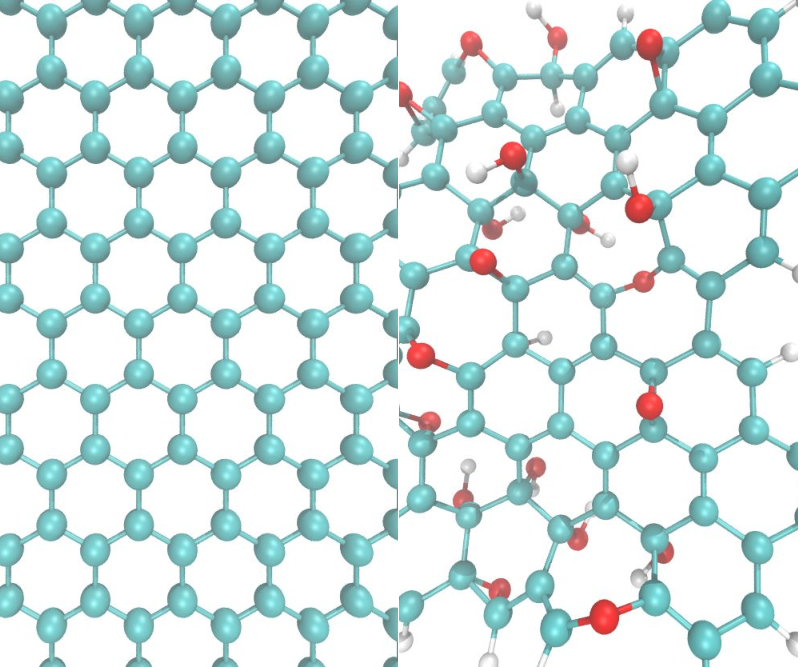
\includegraphics[width=\textwidth]{figs/graphene.pdf}
  \caption{graphene}\label{fig:graphene}
  \end{subfigure}
  \begin{subfigure}{0.45\textwidth}
  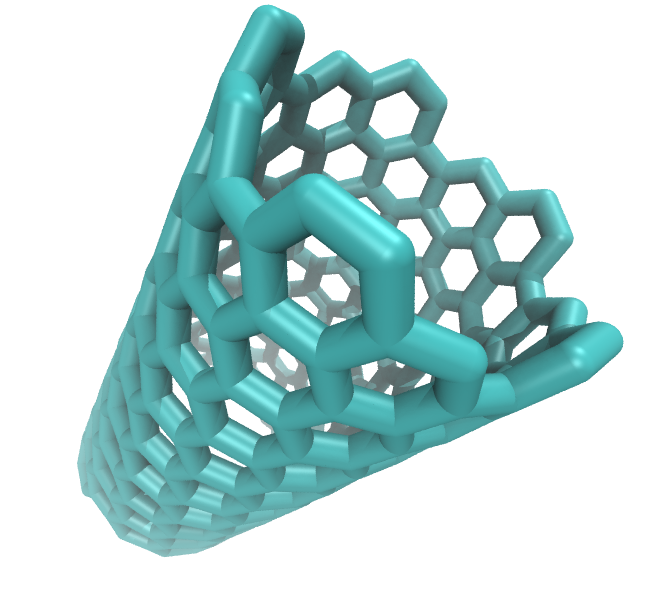
\includegraphics[width=\textwidth]{figs/cnt.png}
  \caption{carbon nanotube}\label{fig:cnt}
  \end{subfigure}
  \begin{subfigure}{0.45\textwidth} % https://america.iza-structure.org/IZA-SC/framework_3d.php?STC=LTA
  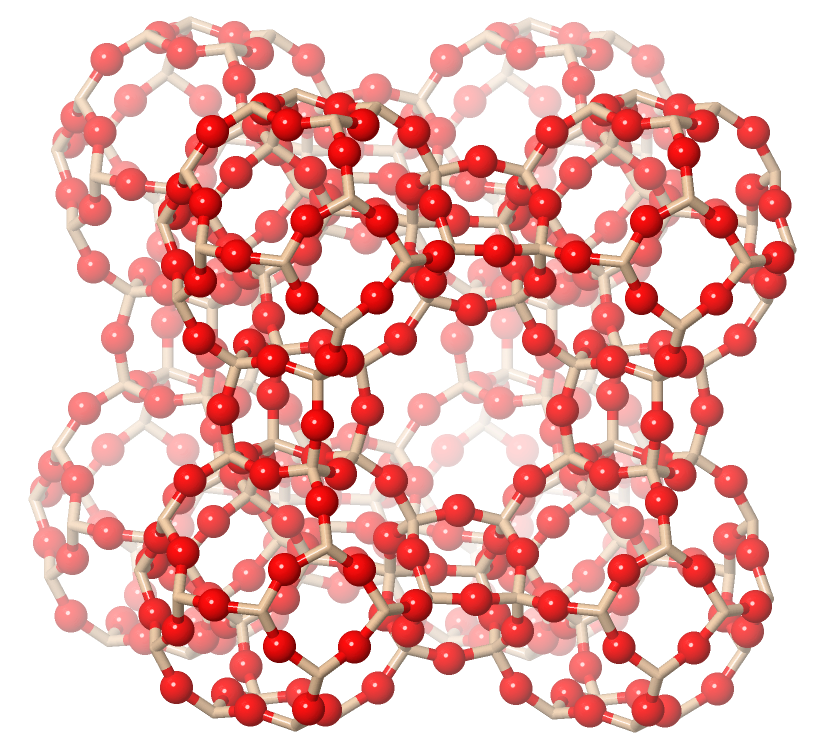
\includegraphics[width=\textwidth]{figs/zeolite.png}
  \caption{zeolite, ZK-4}\label{fig:zeolite}
  \end{subfigure}
  \begin{subfigure}{0.45\textwidth}
  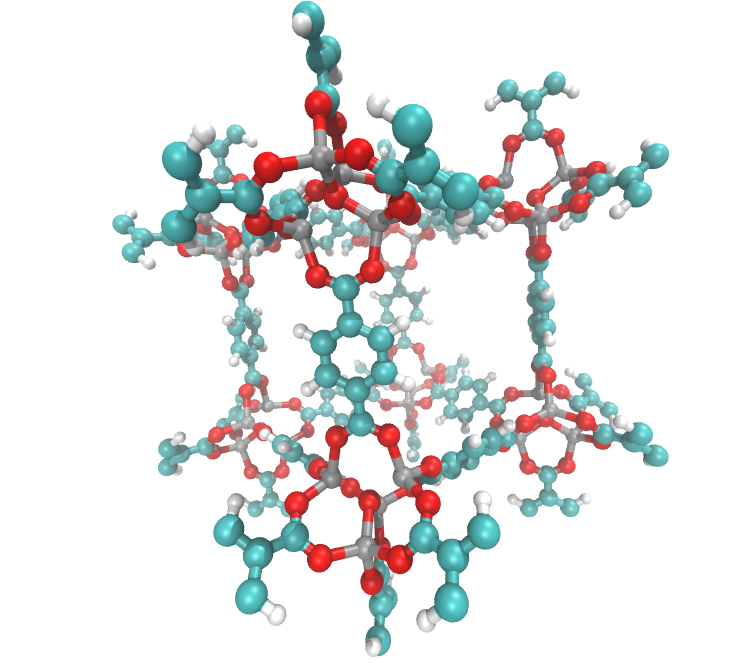
\includegraphics[width=\textwidth]{figs/mof.png}
  \caption{metal organic framework, MOF-5}\label{fig:mof}
  \end{subfigure}
  \caption{(a) Pristine graphene (left) and graphene oxide (right) are atomically thick,
  offering the potential for high permeabilities. (b) Carbon nanotubes exhibit extemely
  fast water transport due to their hydrophobic interiors. (c) Zeolites, like ZK-4 
  shown here, possess cage-like structures that can trap solutes. (d) Metal organic
  frameworks are flexible, porous structures capable of selective adsorption. }\label{fig:nanostructured_materials}
  \end{figure}

  \textit{Graphene and graphene oxide}: Ultrathin-film graphene and graphene oxide membranes
  are an active area of research because they are atomically thick materials and therefore 
  offer potential for extremely high permeability membranes.~\cite{humplik_nanostructured_2011} 
  The tightly packed aromatic network of $sp^2$ hybridized carbon atoms that make up 
  graphene sheets precludes the passage of even the smallest monoatomic species, helium.~\cite{bunch_impermeable_2008}
  Controllably-sized pores have been created in pristine graphene by plasma etching
  and by charged particle bombardment.~\cite{surwade_water_2015,russo_atom-by-atom_2012}
  Graphene oxide (GO), a highly oxidized modification of graphene, consist of epoxy,
  hydroxyl and carboxylate functional groups.~\cite{hegab_graphene_2015}
  Many groups study GO membranes because they have improved antibacterial properties 
  over graphene, leading to less membrane fouling, and because their functionality can be
  modified in order to achieve solute-specific separations.~\cite{liu_antibacterial_2011,he_bioinspired_2013}
  
  Multilayered GO membranes have shown considerably more progress than their single-layered
  counterparts because their synthesis procedures are low cost and scalable.~\cite{zhang_size-controlled_2009} 
  Despite their promise, scalable synthesis of monolayer graphene and GO membranes without
  introducing microscopic, performance degrading defects has not yet been achieved.~\cite{cohen-tanugi_multilayer_2016,wei_multilayered_2018} GO sheets are particularly easy to make into 
  multilayered membranes since they stack on top of each other,
  held together by hydrogen bonds.~\cite{homaeigohar_graphene_2017} The potential of 
  graphene and GO membrane certainly merits their continued exploration. Many groups are still
  working in order to work on better control and standardization of their synthesis, improving
  their designability for specific separations, and further improving their scalability.~\cite{wei_multilayered_2018}  
  
  \textit{Carbon nanotubes}: Carbon nanotubes (CNTs) have shown promise as aqueous 
  separations membranes due to unprecedentedly fast water transport.\cite{humplik_nanostructured_2011}
  CNTs are an allotrope of carbon consisting of nested graphitic cylinders.~\cite{iijima_helical_1991}
  Functionalization of the CNT pore entrances can potentially lead to highly selective 
  separations.~\cite{fornasiero_ion_2008} One can control CNT diameters down to 0.5 nm 
  in size which has inspired the creation of CNT membranes for reverse osmosis 
  applications.~\cite{sun_creating_2000} 
  
  Molecular dynamics simulations have predicted and experiments have confirmed that 
  CNTs are extremely fast transporters of water.~\cite{hummer_water_2001,joseph_why_2008}
  MD simulations by Kalra \textit{et al.} predicted water transport at rates comparable
  to the transmembrane protein aquaporin-1.~\cite{kalra_osmotic_2003} Experiments have 
  exhibited water transport rates orders of magnitude higher than predictions by 
  continuum modeling.~\cite{holt_fast_2006} This enhancement has been explained as a 
  result of nearly friction-less single-file water flow through the hydrophobic CNT 
  interiors.~\cite{kalra_osmotic_2003}
  
  Practically, dispersing and aligning CNTs into a polymer matrix is extremely
  difficult because they tend to agglomerate due to van der Waals forces.~\cite{sahoo_polymer_2010}
  Some work has been to functionalize the carbon nanotubes in order to better incorporate 
  them, however facile incorporation at scale remains a challenge yet to be overcome.~\cite{kim_polysulfone_2007}
  
  \textit{Zeolites}: Zeolite membranes offer the potential for permeabilities 
  comparable to ultrafiltration, with selectivities as good as NF and RO.~\cite{hoek_nanotechnology-based_2014}
  Zeolites have highly uniform nm-sized crystalline structures with cage-like
  cavities that allow movement and trapping of small solutes. The crystalline 
  frameworks are typically formed by networks of silicon and/or aluminum each 
  attached to 4 oxygen atoms in a tetrahedral arrangement.~\cite{auerbach_handbook_2003}
  One can replace the silicon and aluminum atoms via ion exchange in order
  to control the size of the cavities and hence its molecular-seiving properties.~\cite{li_novel_2007}
 
  A number of studies have tested the permeability and sodium salt rejection
  of various zeolite membranes, however their high permeabilities typcially come
  at the cost of low selectivities and vice versa.~\cite{li_desalination_2004,duke_seawater_2009}
  Zeolite-coated ceramic membranes have shown the most promise for RO applications
  because of their mechanical stability under high applied pressure and chemical
  stability for withstanding disinfectants.~\cite{pendergast_review_2011}
  Unfortunately, zeolites are prone to defects in their crystalline structure which 
  would require substantial modification to the traditional synthesis procedures
  in order to fix.~\cite{kumakiri_application_2000}

  \textit{Metal organic frameworks}: Finally, metal organic frameworks (MOFs) have been
  recently introduced to the field of aqueous separations. MOFs are highly porous and 
  flexible crystalline structures made of metal clusters coordinated to organic 
  ligands.~\cite{furukawa_chemistry_2013} Purification of waste streams using MOFs 
  are typically achieved by selective adsorption or catalytic degradation.~\cite{li_metalorganic_2012}
  There is a much wider breadth of research into MOFs as gas separation membranes 
  because they tend to be unstable in water.~\cite{feng_construction_2013} But a new
  generation of water-stable MOFs is making it possible to use them in 
  aqueous separations.~\cite{wang_ultrastable_2015} 

  Recently, MOFs have been applied towards the removal of a number of common water 
  contaminants including dyes, pesticides, endocrine disruptors, and pharmaceuticals.
  \cite{zhang_fabrication_2015,seo_adsorptive_2015,li_metalorganic_2015,hasan_adsorptive_2012}
  Although aqueous MOF separations are theorized to surpass the performance 
  of conventional membrane separations, it is still a budding field. The stability and
  reusability of the material must be guaranteed before they can be implemented
  at scale.~\cite{dias_towards_2015}
  
  \section{Cross-linked Self Assembled Liquid Crystal Membranes for Selective Aqueous Separations}
  
  Amphiphilic molecules that self-assemble to form ordered nanostructures have shown
  potential as nanoporous membranes. People are particularly interested in 
  self-assembled materials because they offer the potential of uniform-sized pores
  and tunable chemical and physical properties.~\cite{werber_materials_2016}
  There are two major classes of self-assembled amphiphilic materials being studied
  for separation applications: block copolymers and liquid crystals.
   
  Block copolymers contain more than one distinct repeating unit which facilitates 
  the formation of self-assembled structures based on differences in the subunit 
  amphiphilicity.~\cite{jackson_nanoporous_2010} Block copolymer membranes typically 
  have pores on the order of 5-50 nm which makes them useful for UF applications, 
  however there is progress being made towards smaller pores in the NF regime.~\cite{gu_tailoring_2015}
  
  Under the right conditions, the shape and amphiphilic character of liquid 
  crystal monomers drives their self-assembling into ordered nanostructures with
  uniform-sized pores on the order of 1 nm in size.~\cite{gin_polymerized_2008}
  As shown in Figure TBD, monomer 1 will form the inverted hexagonal phase 
  (H\textsubscript{II})~\cite{smith_ordered_1997} while monomer 2 will form the 
  bicontinuous cubic phase (Q\textsubscript{I})~\cite{carter_glycerol-based_2012}
  The tails have vinyl groups which can be cross-linked for mechanical strength.

  In this work we attempt to understand how one can design liquid crystal-based
  self-assembled nanostructures for use as alternative membranes for highly selective 
  aqueous separations. We chose to study liquid crystals because they are already 
  suitable as NF membranes and there has been sufficient experimental 
  characterization that we can use as benchmarks for our studies.~\cite{gin_polymerized_2001,feng_scalable_2014,feng_thin_2016}
  
  \begin{figure}
  \centering
  \includegraphics[width=\textwidth]{figs/lc_phases.pdf}
  \caption{The amphiphilic character of liquid crystal monomers drives their
  self-assembly into various nanostructured phases with uniform sized pores. 
  The hydrophilic components of the monomers line the aqueous pores, offering
  potential for selective interactions with passing solutes. The monomer on 
  the top left will form the inverted hexagonal (H\textsubscript{II})
  phase which is composed of aligned cylindrical pores packed in a hexagonal 
  array. This geometry is theoretically ideal for high throughput transport. 
  The monomer on the right will for the type I bicontinuous cubic phase
  (Q\textsubscript{I}) in either the Ia3d (gyroid) or Pn3m (diamond) space group.
  Although the Q\textsubscript{I} phase has a much more tortuous network of 
  pores than the H\textsubscript{II}, which should lower its relative permeabily,
  its synthesis is much more practical because it does not require alignment of
  the nanostructured mesophases.
  }\label{fig:lc_phases}
  \end{figure}

  \subsection{The H\textsubscript{II} Phase}
   
  The H\textsubscript{II} phase is characterized by hexagonally packed, uniform-sized
  and straight pores.~\cite{smith_ordered_1997} The hydrophilic head groups aggregate
  in the pore centers to create cylindrical aqueous channels. These pore channels are
  lined with the chemical functionality of the LLC monomers and have the potential to
  interact with solutes in a chemically-dependent manner. The inhomogeneity of the 
  pores suggests that the effective pore size may depend on the solute. Both the size,
  shape and chemical functionality will influence how a solute partitions within the 
  membrane. In theory, this pore topology and geometry is ideal for high flux and 
  highly selective separations.
  
  Unfortunately, it is a difficult task to align the self-assembled hexagonal
  mesophases into continuous pores that traverse the thickness of the membrane.
  Although the membranes have shown high experimental selectivity, their flux has been
  very low due to misalignment of the hexagonal mesophases.~\cite{zhou_supported_2005}
  
  Considerable recent efforts have made progress towards the macroscopic
  alignment of the hexagonal mesophases. Feng \textit{et al.} leveraged the magnetic 
  anisotropy of the columnar mesophases in order to control their alignment with a 
  magnetic field.~\cite{feng_scalable_2014} This study showed an 85-fold increase in
  ionic conductivity in the aligned versus unaligned state, demonstrating a huge 
  increase in feasibility as an industrial membrane. Feng \textit{et al.} also used
  an approach called soft confinement which takes advantage of the hexagonal columns'
  preference towards anchoring perpendicular to either a PDMS or glass substrate.~\cite{feng_thin_2016}
  Finally, Feng \textit{et al.} designed a third technique which uses a structure
  directing molecule in order to template the assembly of a fatty acid 
  molecule into ordered columnar phases.~\cite{feng_highly_2017} These advances 
  have revived research interest in H\textsubscript{II} phase membranes.
  
  \subsection{The Q\textsubscript{I} Phase}
  
  The bicontinuous cubic, or Q\textsubscript{I} phase, is a class of nanostructured
  phases characterized by a network of 3 dimensionally interconnected pores.~\cite{hyde_bicontinuous_1996}
  Aside from its tortuous pore architecture, it shares the uniform size and complex 
  topological features of the H\textsubscript{II} phase which lends itself to highly
  selective separations. Although water and solutes must follow a longer path in order
  to pass through Q\textsubscript{I} membranes, they are more practical to synthesize
  than the H\textsubscript{II} phase because the mesophases do not require alignment.~\cite{zhou_new_2007}
  
  % Figure here  
  
  The space group of the Q\textsubscript{I} phase configuration formed by
  monomer 1 is uncertain and thought to be either Pn3m or Ia3d. Six Q phase
  architectures have been identified in small molecule amphiphile systems.~\cite{mariani_cubic_1988}
  Of these, only 4 are consistent with diffraction data generated by the gemini
  surfactant used here: Q$^{230}$ (Ia3d), Q$^{224}$ (Pn3m), Q$^{229}$ (Im3m) and Q$^{212}$ 
  (P4\textsubscript{3}32), all of type I configuration~\cite{pindzola_cross-linked_2003}
  The presence of $1 / \sqrt{6}$ and $1 / \sqrt{8}$ peaks rules out the
  Q$^{227}$ (Fd3m) and Q$^{223}$ (Pm3n) configurations. The Pn3m and Ia3d architectures
  are most commonly observed experimentally.~\cite{mariani_cubic_1988,wiesenauer_nanoporous_2012}
%    \item The most likely phase is the type I Q$^{230}$ (Ia3d) because it is the
%    most common phase observed between lamellar and hexagonal phases and the
%    monomeric alkyltrimethylammonium salts used to synthesize the gemini LCs
%    exhibit clear Ia3d symmetry.
%MRS3: is this last bit necessarily implied (symmetry of phasae bby symmetry of salt)?  It's not clear to me it is.
%BJC3: Yea, I don't know, this was stated in a Gin paper

  Due to its more facile synthesis, there has been significantly more development
  of Q\textsubscript{I} phase membranes. The first generation of Q\textsubscript{I}
  membranes was made by the self-assembly of a gemini phosphonium monomer in 
  water.~\cite{pindzola_cross-linked_2003} Hatakeyama \textit{et al.} improved the 
  industrial viability of Q\textsubscript{I} phase membranes by using a gemini 
  ammonium monomer which is both easier and cheaper to synthesize.~\cite{hatakeyama_nanoporous_2010}
  Free standing films of both first and second generation Q\textsubscript{I} phase 
  membranes cannot withstand high pressure. Because solution casting was ineffective,
  Zhou et. al used a hot-pressing method to make mechanically strong membranes which
  involves heating the initial monomer mixture to 70\degree C and pressing it with 12
  tons of force into a thick microporous, hydrophilic polymer support.~\cite{zhou_new_2007}
  The most recent generation of Q\textsubscript{I} membranes uses an imidazolium-based
  gemini LLC monomer which is capable of being solution cast into defect-free thin films 
  on porous supports. This improvement resulted in a ten-fold increase in flux while 
  retaining selectivities similar to earlier generations.~\cite{carter_glycerol-based_2012}
  
  %BJC: figure with different generation Q1 monomers
  
  State of the art Q\textsubscript{I} membranes offer selectivities that
  are competitive with existing commercial technologies. When separating organic
  solutes from NaCl, Q\textsubscript{I}-phase membrane filtration experiments have
  shown selectivity 2--3 times higher than commercial RO and 6--12 times higher 
  than commercial NF membranes.~\cite{dischinger_application_2017} Their water 
  lies between commercial RO and NF membranes. There is work being done to reduce 
  the thickness of the selective layer in order to increase permeability. 

  %\section{Atomistic Molecular Simulation of LLC Membranes}
  \section{Modeling Membrane Separations}
  
  %BJC2: taken from stochastic transport paper.
  Mathematical descriptions of transport in complex separations membranes are a
  powerful way to understand mechanisms and formulate design principles.
  \cite{vinh-thang_predictive_2013,geens_transport_2006,darvishmanesh_mass_2016}
  The complexity of a well-fit model generally parallels the complexity of the
  transport mechanism being studied, as well as the transport information the
  model conveys. In dense homogeneous membranes, the solution-diffusion model
  can extract diffusion and partition coefficients and has successfully
  predicted solute transport rates.~\cite{wijmans_solution-diffusion_1995}
  Analogously, pore-flow models yield predictions of diffusion coefficients and
  solute transport rates in nanoporous membranes.~\cite{paul_diffusive_1974}
  Modern single particle tracking approaches have taken researchers beyond
  continuum modeling allowing them to characterize complex diffusive
  behavior.~\cite{manzo_review_2015} At the molecular level, one can use
  molecular dynamics (MD) simulations to study both single particle dynamics
  and bulk transport properties with atomic-level
  insight.~\cite{coscia_chemically_2019,maginn_best_2018} All of these
  approaches facilitate generation of hypotheses about the molecular origins of
  separations by attempting to give a more intuitive understanding of how
  solutes move as a function of their environment, in turn suggesting
  experiments that could be performed.
  
  This thesis uses the high level of detail afforded by MD simulations in
  order to understand solute transport within LLC membranes with molecular 
  detail. Before diving into an atomistic model, we offer a brief survey of 
  the most popular macroscopic treatments in order to highlight how a 
  nanoscopic perspective offered by atomistic modeling may be better suited to 
  understanding how to design the next generation of LLC membranes.

  \subsection{Macroscopic Treatments}
  
  The most widely used approaches to modeling transport in membranes of all types
  are based on macroscopic theory. In this section we will discuss the two prevailing
  theories: the pore flow model and the solution-diffusion model.
  
  Membrane permeation is the result of a chemical potential gradient, $\frac{d\mu_i}{dx}$.
  The flux of component $i$ is proportional to this gradient:
  \begin{equation}
    J_i = -L_i \frac{d\mu_i}{dx}
  \end{equation}
  where $L_i$ is a coefficient of proportionality.~\cite{wijmans_solution-diffusion_1995}
  $L_i$ is an intrinsic materials property dependent on the chemical makeup of
  the membrane and usually determined via experiment. Chemical potential gradients
  can be induced by concentration, pressure, temperature
  and electromotive forces. We will limit our discussion to concentration and pressure
  gradients because these are primarily forces used for separations with the types of 
  membranes we will be studying.

  For pressure driven membrane processes, water flux through both porous and 
  amorphous membranes can be described by
  \begin{equation}
  J_w = A(\Delta P - \Delta \pi_m)
  \end{equation}
  where $J_w$ is volumetric water flux, $A$ is the water permeability coefficient,
  $\Delta P$ is the applied hydraulic pressure and $\Delta \pi_m$ is the 
  trans-membrane osmotic pressure difference. Estimates of the water permeability 
  coefficient and the solute flux are dependent on how one models flow through the 
  membrane.

  In porous membrane architectures, water and solute flux are modeled as laminar flow
  through cylindrical pores. The derivation of flux follows Hagen-Poiseuille flow with 
  inclusion of morphological characteristics:~\cite{baker_membrane_2012}
  \begin{equation}
    A = \frac{\varepsilon r_p^2}{8\mu\delta_m}
  \end{equation}
  where $\varepsilon$ is the surface porosity, $r_p$ the pore radius, $\delta_m$ the
  membrane thickness, and $\mu$ the solution viscosity. Solute flux, $J_s$ is related
  to $J_w$ but scaled by the empirically measured permeate concentration:
  \begin{equation}
    J_s = c_p J_w
  \end{equation}
  Analytical expressions for solute flux, such as the Donnan Steric Pore Model (DSPM), 
  are typically quite complicated because they attempt to incorporate more system features
  leading to less assumptions.~\cite{bowen_modelling_2002}
  
  Solute rejection is the quantity frequently used to characterize the performance of a 
  filtration membrane. Under the pore flow model, solutes with radii smaller than the 
  pore will not pass through the membrane. A membrane with uniform-sized pores smaller
  than the solute being targeted for separation should have a solute flux of 0. However,
  in practice, most membranes have a distribution of pore sizes, some large enough to
  allow solutes to pass. Therefore, separation performance is typically characterized
  in terms of solute rejection, $R$. 
  \begin{equation}
     R = 1 - \frac{c_p}{c_f}
  \end{equation}
  where $c_p$ and $c_f$ are the concentrations of the rejected species in the permeate
  and feed respectively. The DSPM has been used to directly predict 
  rejection.~\cite{hatakeyama_water_2011,bowen_modelling_2002}
  
  % BJC: mention does not enter Brownian regime
  In amorphous membranes, water and solute flux are modeled using the solution-diffusion 
  model. It is hypothesized that water and solute molecules partition into the
  membrane and diffuse across the polymer matrix due to a chemical potential gradient
  and then desorb into the permeate. The product of a component's solubility and 
  diffusivity is commonly referred to as its permeability, $P$.~\cite{wijmans_solution-diffusion_1995}
  $P$ is an intrinsic material property and is thus independent of membrane thickness.  % BJC: is intensive a more appropriate word than intrinsic?
  The water permeability coefficient, $A$, \textit{is} dependent on thickness, $\delta_m$,
  and can be formulated in terms of the pure water permeability, $P_w$.
  \begin{equation}
    A = \frac{P_wV_w}{\delta_mR_gT}
  \end{equation}
  where $V_w$ is molar volume of water, $R_g$ is the universal gas constant and $T$ is
  absolute temperature. Solute flux is modeled as:
  \begin{equation}
    J_s = \frac{P_s}{\delta_m}\Delta c_m = B\Delta c_m
  \end{equation}
  where $B$ is a solute permeability coefficient and $\Delta c_m$ is the concentration
  difference across the selective membrane layer.~\cite{geise_fundamental_2014}
  Under these assumptions, rejection can be reformulated as
  \begin{equation}
    R = \frac{A}{A + B}
  \end{equation}
  which approaches unity as the solute flux tends towards zero.~\cite{van_der_bruggen_review_2003}
  
  These equations provide a somewhat limited perspective on the molecular details
  of transport. The pore flow model neglects molecular level interactions with the 
  membrane and assumes all transport occurs within the cylindrical pore region. In
  this work, we will show that solutes are not confined to the ``pore region" and 
  that motion is heavily influenced by interactions with membrane. The 
  solution-diffusion model assumes that solutes undergo Brownian motion. As will
  be discussed, solutes appear to undergo subdiffusive behavior on short timescales. 
  Therefore, we may need a more descriptive theory in order to appropriately address
  questions of membrane design.
  
%MRS3: think about if there is a way to better connect the information
%above to the work carried out in the thesis, besides just ``we need a better theory''.

  \subsection{Atomistic Molecular Simulation of LLC Membranes}  
  
  %BJC: following two paragraphs taken from first paper.
  %BJC2: Could probably reorganize the sentences of these next two paragraphs 
  % to flow better with rest of intro.
  %BJC2: These next two paragraphs might function better in previous section.
%  Our current understanding of the molecular details of LLC polymer membranes'
%  nanostructure is not sufficient to be able to precisely design them for
%  specific separations. Dischinger \textit{et al.}~attempted to use an empirical model
%  that correlates the physiochemical properties of the counterion used in a
%  Q\textsubscript{I}-phase LLC membrane to solute rejection\cite{dischinger_effect_2017}.
%  Although their model showed some qualitative agreement with experiment, the
%  quality of fit of their model was limited due to complex solute-membrane
%  interactions that could not easily be modeled. Additionally, they observed
%  an unexpected discrepancy in the relationship between uncharged solute
%  rejection and water permeability, which will require a more in-depth knowledge of
%  the difference between solute and solvent transport.
%
%  Over the past 20 years, H\textsubscript{II}-phase LLC polymer membrane
%  studies have been limited primarily to the Na-GA3C11 monomer with some
%  characterization done after minor structural modifications. For example, Resel
%  \textit{et al.}~varied the length of the monomer tails and the counterion used and
%  observed its effect on pore spacing \cite{resel_structural_2000}. In a later
%  study of rejection performance, it was shown that membranes formed by
%  cross-linked Na-GA3C11 in the H\textsubscript{II} phase cannot separate solutes
%  less than 1.2 nm in diameter because the pores are too large.
%  %MRS: this above is interesting, since that seems somewhat inconsistent with the 
%  \cite{zhou_supported_2005} We do not yet understand how to controllably reduce
%  the effective pore size or how to tune the chemical environment in the
%  nanopores of this or related materials for small molecule separations. The only
%  source of predictive modeling for LLC systems have been macroscopic models that
%  likely do not adequately describe transport at these length scales
%  \cite{hatakeyama_water_2011}. Modeling with molecular detail could provide
%  sufficient information about the mechanisms and chemical features to better
%  inform experimental design of similar nanostructured membranes.
  
  A molecular-level understanding of the relationship between monomer structure
  and solute transport can help provide guidelines to reduce the large chemical 
  space available to design monomers for creation of separation-specific membranes. 
  Atomistic MD simulations can provide the required level of detail (Figure 
  \ref{fig:detailed_pore}), assuming the force fields are sufficiently accurate. 
  With such an atomistic model, we can directly observe molecular-level solute 
  transport and suggest governing mechanisms. We can also observe how the choice 
  of head group and counterions interacts with solutes of interest. 

  \begin{figure}[!htb]
  \centering
	\begin{subfigure}{0.45\linewidth}
		\centering
		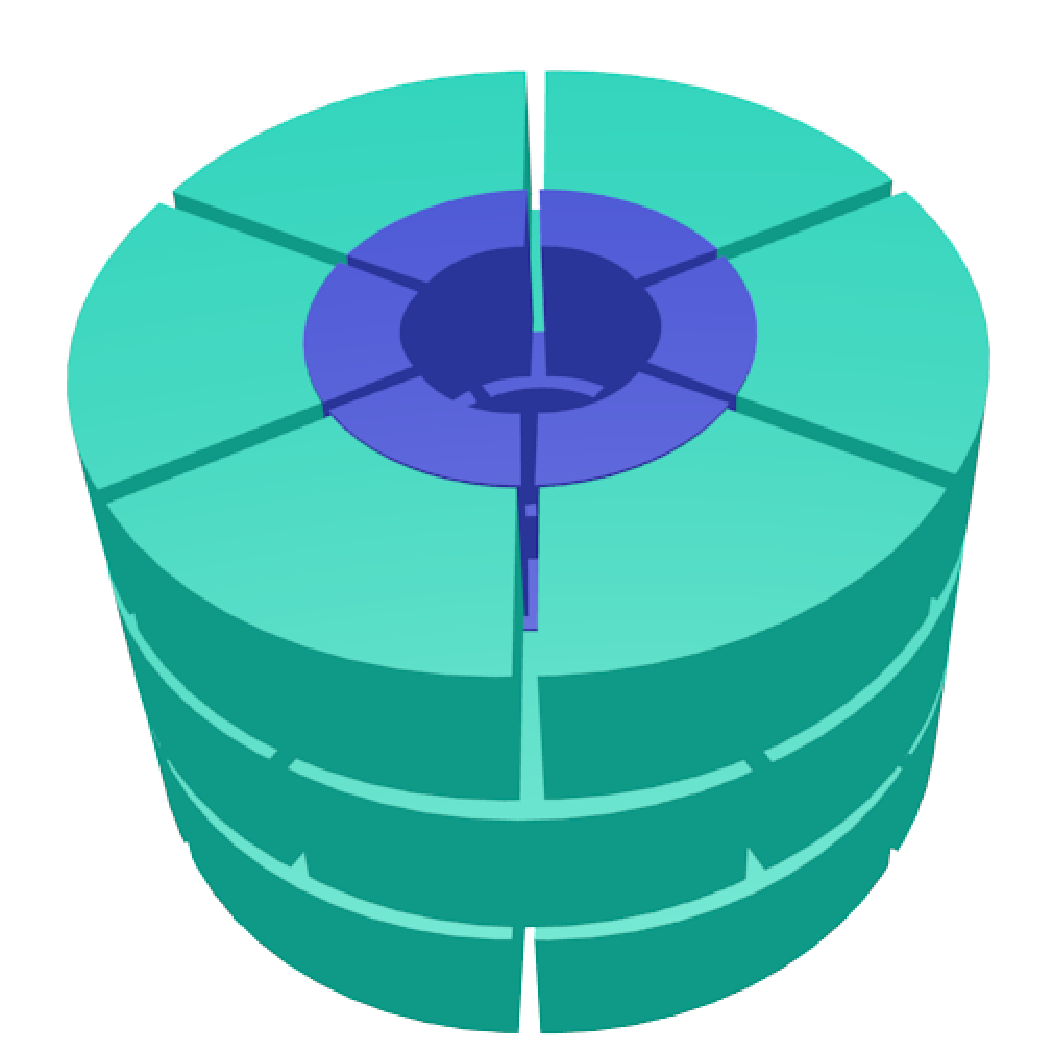
\includegraphics[width=0.6\textwidth]{cartoon_pore.pdf}
		\caption{}~\label{fig:undetailed_pore}
	\end{subfigure}
	\begin{subfigure}{0.45\linewidth}
		\centering
		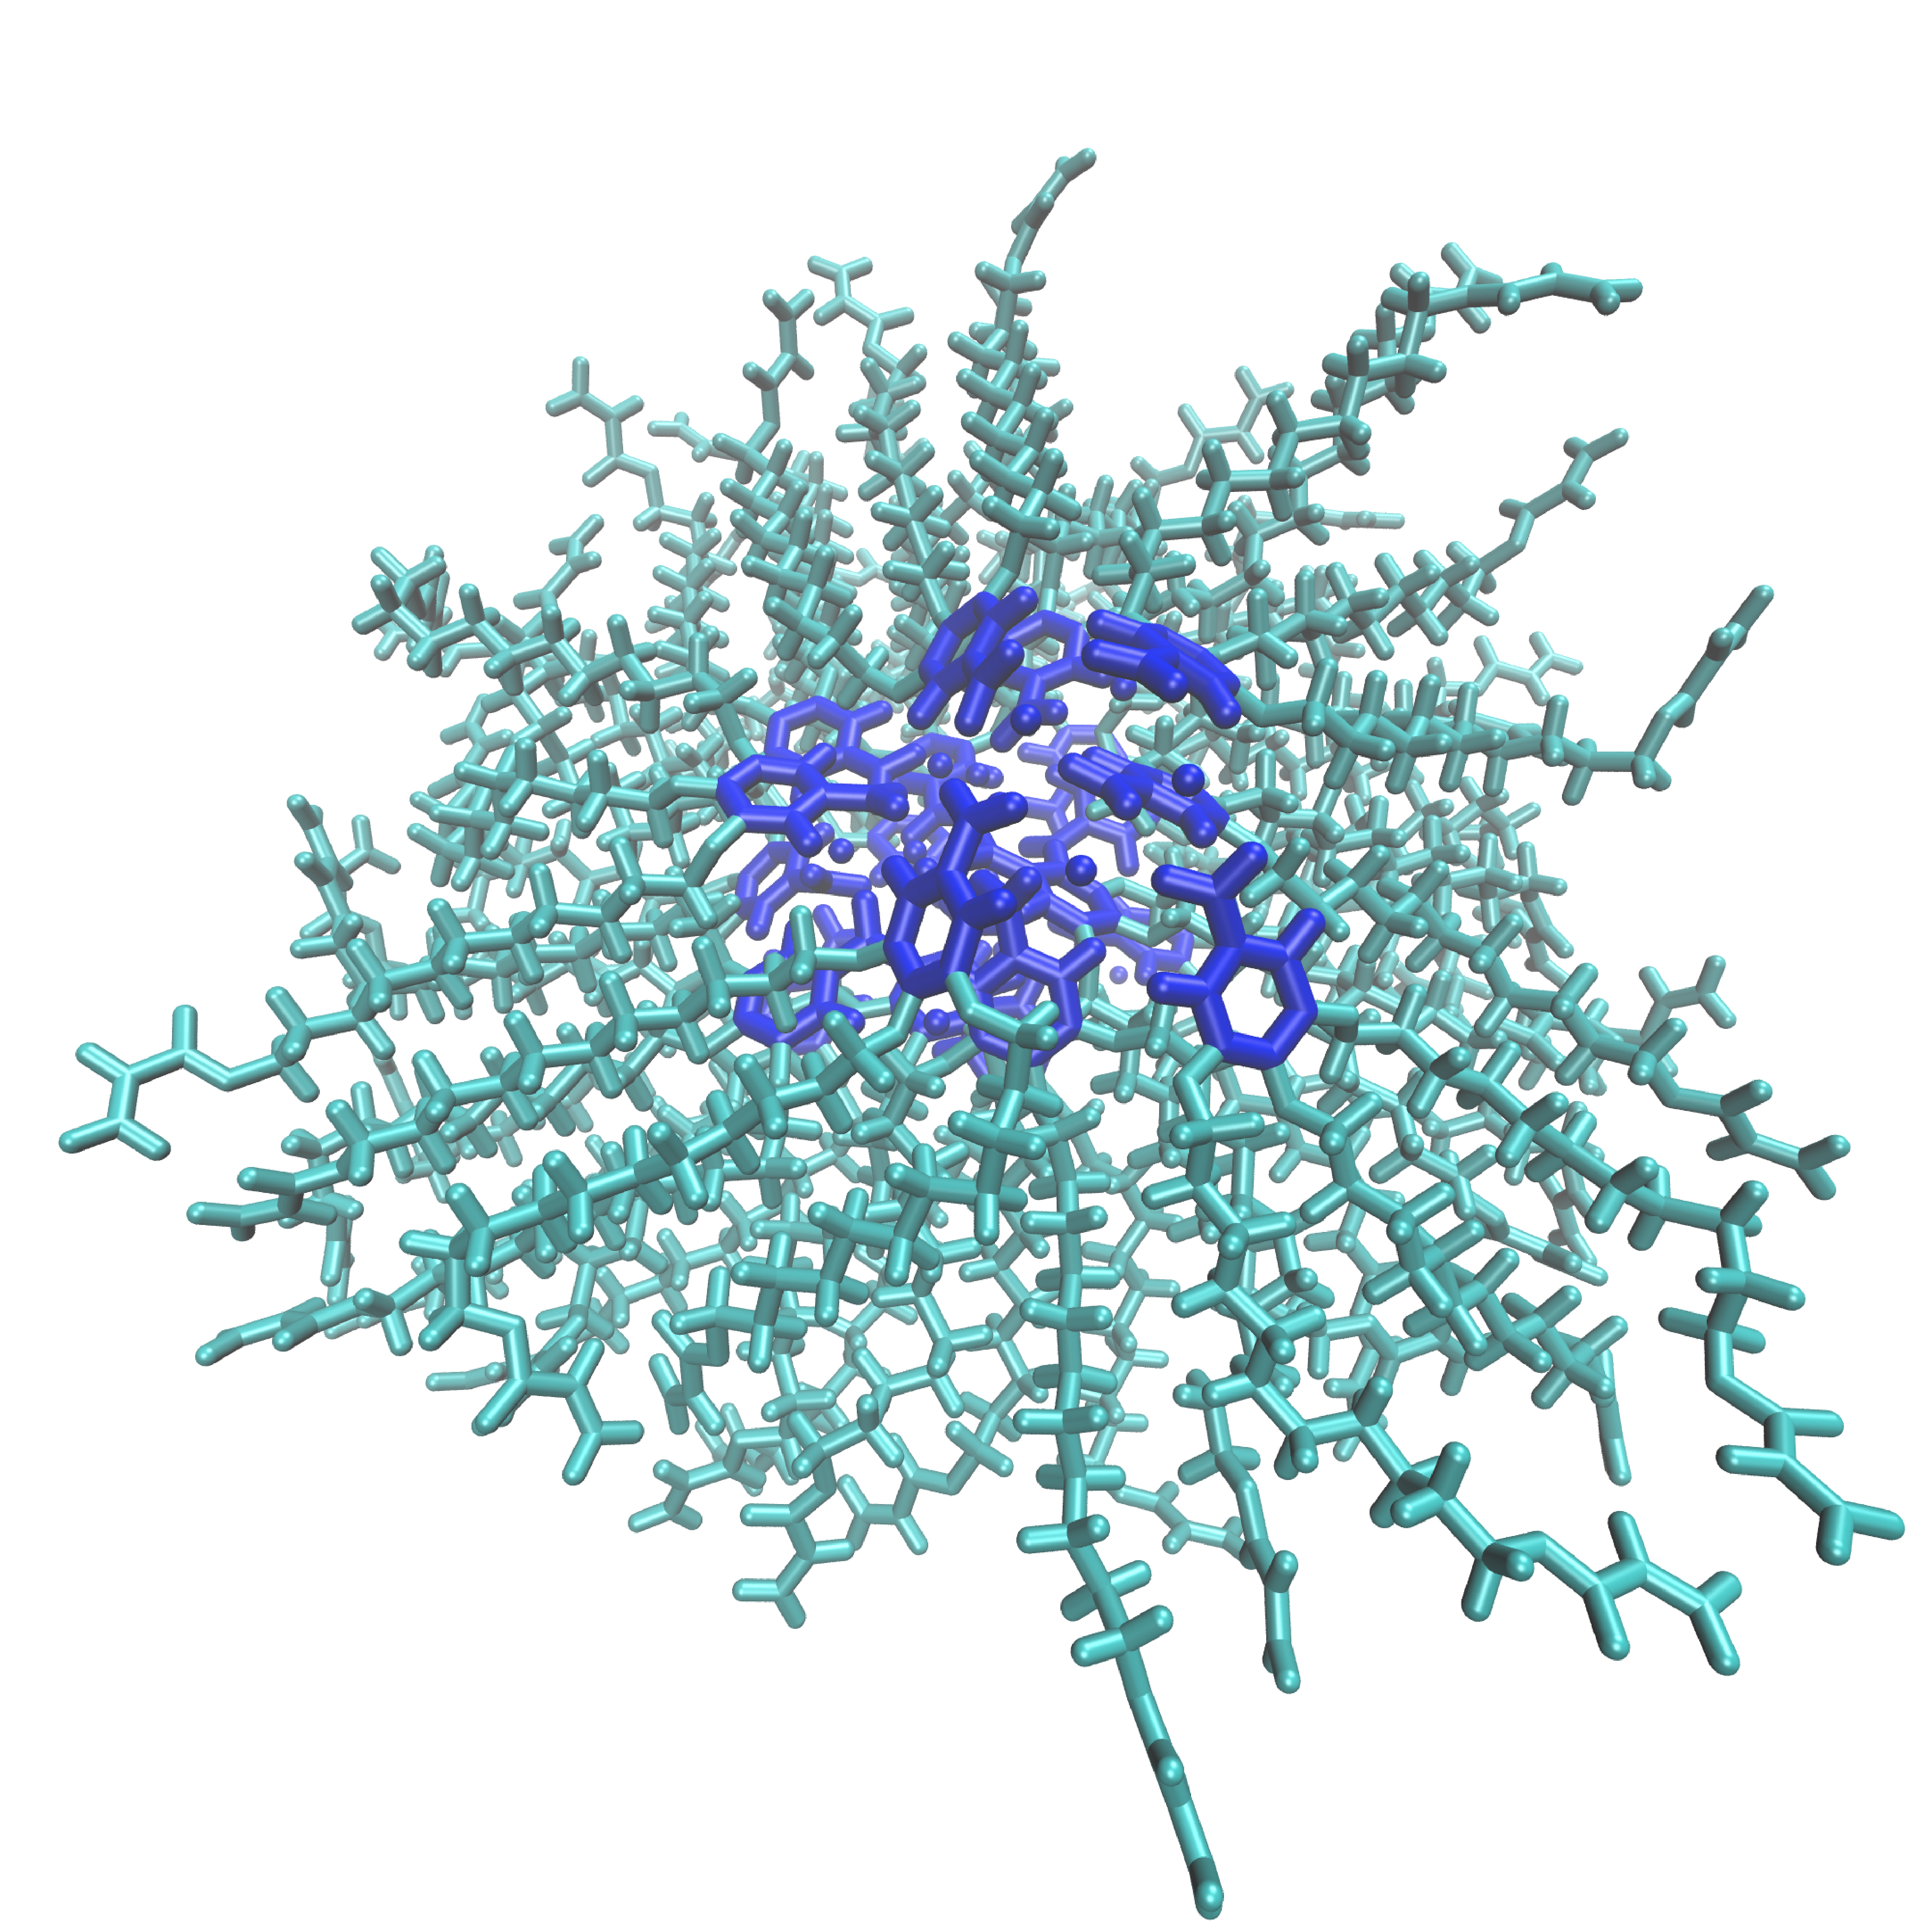
\includegraphics[width=0.6\textwidth]{detailed_pore.pdf}
		\caption{}~\label{fig:detailed_pore}
	\end{subfigure} 
    \caption{(a) Previous understanding of the LLC pores are essentially speculations 
    based on limited chemical and experimental data. (b) We use detailed molecular 
    modeling in this paper in order to appropriately model the pore's complex architecture,
    which is crucial to understanding the mechanism of solute transport. In both 
    pictures, the head group region is colored blue and the tail region is colored cyan.}~\label{fig:detail}
  \end{figure}

  Although the Q\textsubscript{I} phase shows the most promise for practical 
  applications, the focus of this work will be on the H\textsubscript{II}
  phase. The H\textsubscript{II} phase is an easier to geometry to model
  and analyze. We also have detailed structural data which is necessary for 
  validating our model. All of the analysis techniques we use can be equally
  adapted to the more complicated Q\textsubscript{I} phase geometry.
  
  There are few molecular simulation studies which study structure and transport
  in LLC systems. Mondal \textit{et al.} used MD simulations to study the self assembly 
  of gemini surfactants and observed the formation of H\textsubscript{II} and
  Q\textsubscript{I} phases depending on water content.~\cite{mondal_self-assembly_2013}
  Mantha and Yethiraj as well as Roy \textit{et al.} studied the dynamics of confined 
  water in these systems and showed orders of magnitude differences in their motion
  dependent on system geometry.~\cite{mantha_dynamics_2016,roy_water_2016}
  Jackson \textit{et al.} as well as Mantha \textit{et al.} have combined experiment
  with simulation in order to show how the choice of monomer head group counterion 
  regulate water dynamics.~\cite{jackson_ion-specific_2018,mantha_counterion-regulated_2018}
  Sakamoto \textit{et al}. and Nada \textit{et al}. observed the dynamics of water 
  molecules and ions and hypothesized transport mechanisms in a simplified model of
  an LLC nanopore.~\cite{sakamoto_development_2018,nada_transport_2020}

  Because there is relatively sparse coverage of these types of simulation systems in 
  the literature, we have built a detailed molecular model from the ground up. There 
  are four primary research questions that we will address in this work.
  \begin{enumerate}
    \item What is the nanoscopic structure?

    	  Before we can try to understand the molecular mechanisms of solute
    	  transport, we need to ensure that we model the chemical environment
    	  within the nanopores in a way that is consistent with experiment.
    	  We use experimental structural data in order to validate our model and
    	  understand the sensitivity of the model to build parameters.

    \item Which solute-membrane interactions have the greatest influence on transport rates?
    	  
    	  After gaining a detailed picture of the nanopore structure, we can 
    	  feel confident that solutes in this system will experience qualitatively 
    	  similar interactions which are present in a real system. We create independent
    	  systems for each of 20 small polar solutes and observe transport mechanisms
    	  whose dominance is dependent on solute chemical functionality. We characterize
    	  three different trapping mechanisms which lead to subdiffusive transport behavior.
    	  
    \item Can we formulate mechanistic models whose dynamical properties are consistent with our
    molecular simulations and can be used to extrapolate macroscopic behavior which MD simulations cannot.

		  Using our qualitative understanding of the dominant trapping mechanisms,
    	  we develop stochastic time series models which we can use to mimic solute dynamic
    	  behavior on time scales orders of magnitude longer than our simulations. 
    	  We attempt to reproduce both quantitative and qualitative solute trajectory
    	  behavior on MD simulation-length timescales. We then show how we can use our 
    	  most promsiing model in order to connect microscopic transport to macroscopic
    	  flux and selectivity.

    \item How can time series data directly inform us about transport mechanisms?
    	
    	  Although our stochastic models show great promise, their development requires
    	  some qualitative and quantitative understanding of dominant transport
    	  mechanisms. In the final chapter, we use the infinite hidden Markov model in
    	  order to automatically detect and parameterize a unknown number of hidden 
    	  dynamical modes exhibited by solute time series. This more flexible approach
    	  allows us to both infer mechanisms based on differences in dynamical behavior
    	  and generate stochastic trajectory realizations which we can use to predict
    	  flux and selectivity. 
 
  \end{enumerate} 
  
  The next four chapters offer answers to each of the above questions and are adapted from 
  my first author manuscripts at various stages in the publication process as described
  below. The introduction to each adaptation is condensed in order to avoid redundancy and 
  all other sections are left intact. The supporting information documents for each manuscript are
  given in the appendices. \\
  
  %MRS: maybe put supporting information for each chapter at the end of the chapter so it's in one place?
  %BJC3: it makes the numbering a little confusing. I'll see if there's a way around it.

%  \noindent\textit{Chapter 2}: adapted from manuscript entitled ``Understanding the 
%  Nanoscale Structure of Inverted Hexagonal Phase Lyotropic Liquid Crystal Polymer Membranes." 
%  published in the Journal of Physical Chemistry B.~\cite{coscia_understanding_2019} \\
%
%  \noindent\textit{Chapter 3}: adapted from manuscript entitled ``Chemically Selective 
%  Transport in a Cross-Linked H\textsubscript{II} Phase Lyotropic Liquid Crystal Membrane."
%  published in the Journal of Physical Chemistry B.~\cite{coscia_chemically_2019} \\
%    
%  \noindent\textit{Chapter 4}: adapted from a manuscript in review with Physical Review E, entitled 
%  ``Capturing Subdiffusive Solute Dynamics and Predicting Selectivity in Nanoscale Pores
%  with Time Series Modeling". The final manuscript may change based on reviewer feedback. \\
%    
%  \noindent\textit{Chapter 5}: adapted from the draft of a manuscript in preparation with the working
%  title ``Statistical Inference of Transport Mechanisms and Long Time Scale Behavior from Time Series 
%  of Solute Trajectories in Nanostructured Membranes." The content will change as the
%  draft is finalized and after reviewer feedback.
  
  \noindent\textit{Chapter 2}: adapted from Coscia, B. J.; Yelk, J.; Glaser, M. A.; Gin, D. L.; Feng, X.; Shirts,
  M. R. Understanding the Nanoscale Structure of Inverted Hexagonal Phase Lyotropic Liquid Crystal Polymer
  Membranes. J. Phys. Chem. B 2019, 123, 289-309. \\
    
  \noindent\textit{Chapter 3}: adapted from Coscia and Shirts. Chemically Selective Transport in a Cross-Linked 
  H\textsubscript{II} Phase Lyotropic Liquid Crystal Membrane. J. Phys. Chem. B 2019, 123, 6314-6330. \\
    
  \noindent\textit{Chapter 4}: adapted from a manuscript in review with Physical Review E, entitled 
  "Capturing Subdiffusive Solute Dynamics and Predicting Selectivity in Nanoscale Pores
  with Time Series Modeling". The final manuscript may change based on reviewer feedback. \\
    
  \noindent\textit{Chapter 5}: adapted from the draft of a manuscript in preparation with the working
  title "Statistical Inference of Transport Mechanisms and Long Time Scale Behavior from Time Series 
  of Solute Trajectories in Nanostructured Membranes." The content will change as the
  draft is finalized and after reviewer feedback.
